In this section we document the matrix element output distributions 
comparing data to the signal and background predictions, corresponding to 
\intlumi data.


%%%%%%%%%%%%%%%%%%%%%%
\begin{figure}[!ht]
\begin{center}
   \subfigure[]{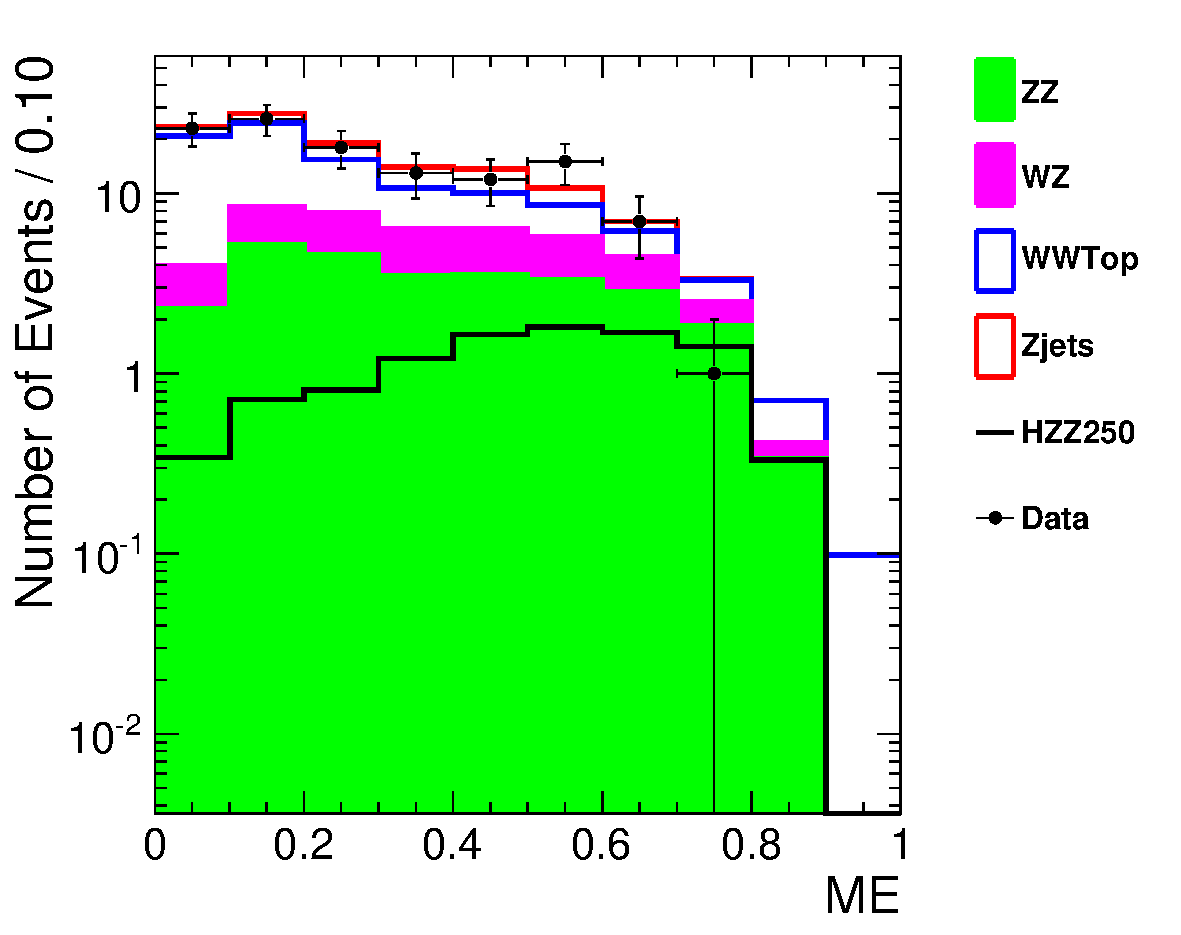
\includegraphics[width=0.4\textwidth,angle=0]{figures/ME_mH250_ee_stack_log.pdf}} 
   \subfigure[]{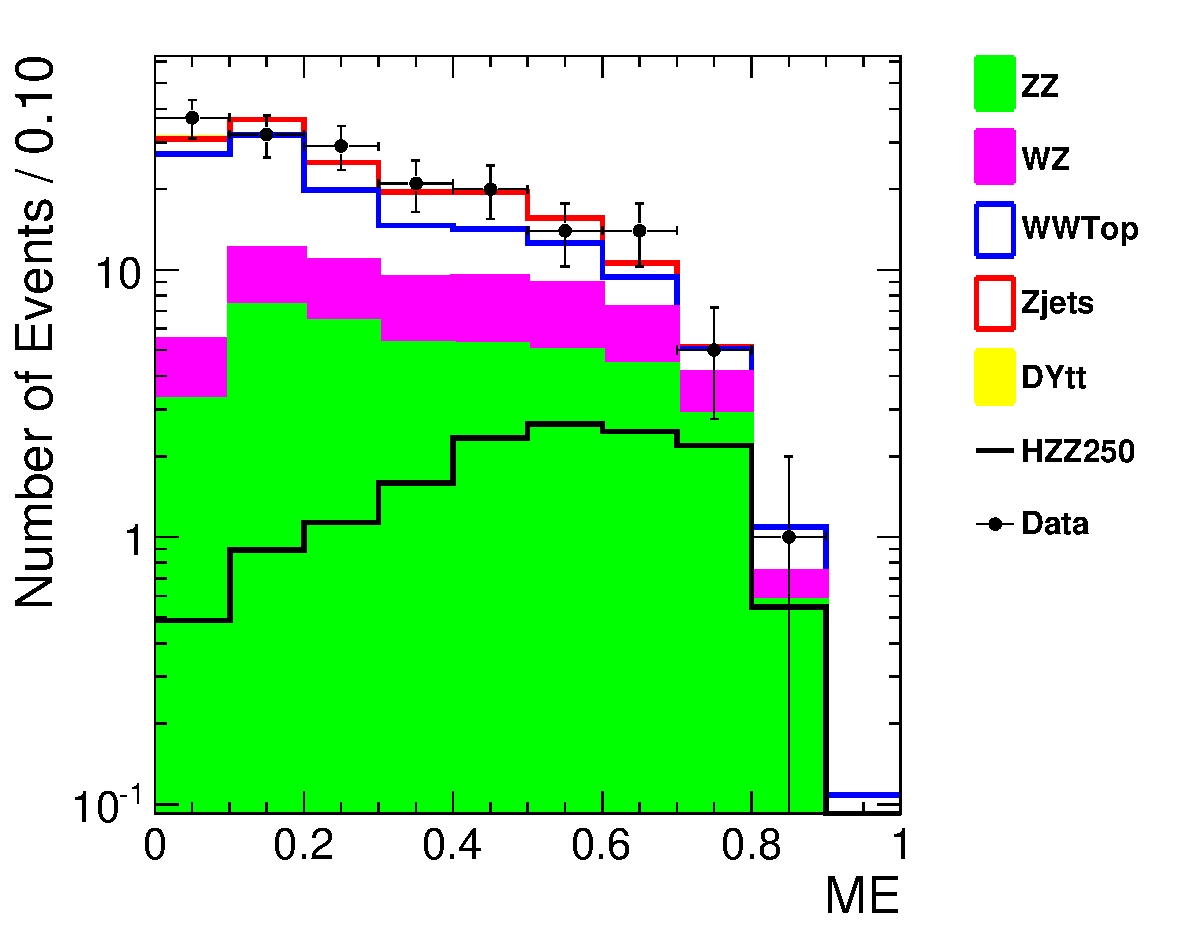
\includegraphics[width=0.4\textwidth,angle=0]{figures/ME_mH250_mm_stack_log.pdf}} \\ 
   \caption{The matrix element output distribution for Higgs signal and background events 
for \mHi=250 $\GeVcc$ in ee (a) and $\mu\mu$ final state (b) after the higgs dependent selections. 
The distributions are normalized to \intlumi with the background scaled by the data-to-mc ratios derived from data.}
   \label{fig:histo_me_250_5fb}
\end{center}
\end{figure}

\begin{figure}[!ht]
\begin{center}
   \subfigure[]{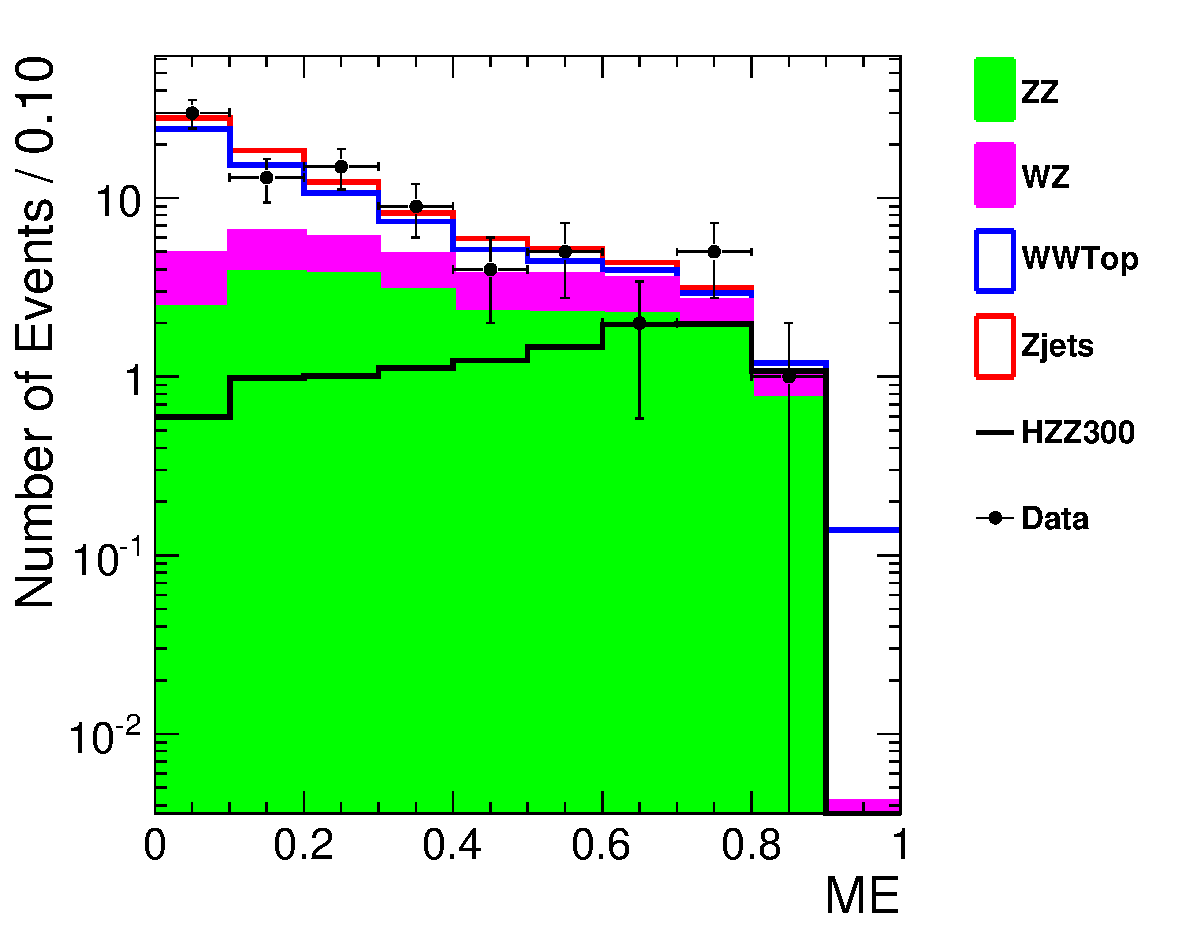
\includegraphics[width=0.4\textwidth,angle=0]{figures/ME_mH300_ee_stack_log.pdf}} 
   \subfigure[]{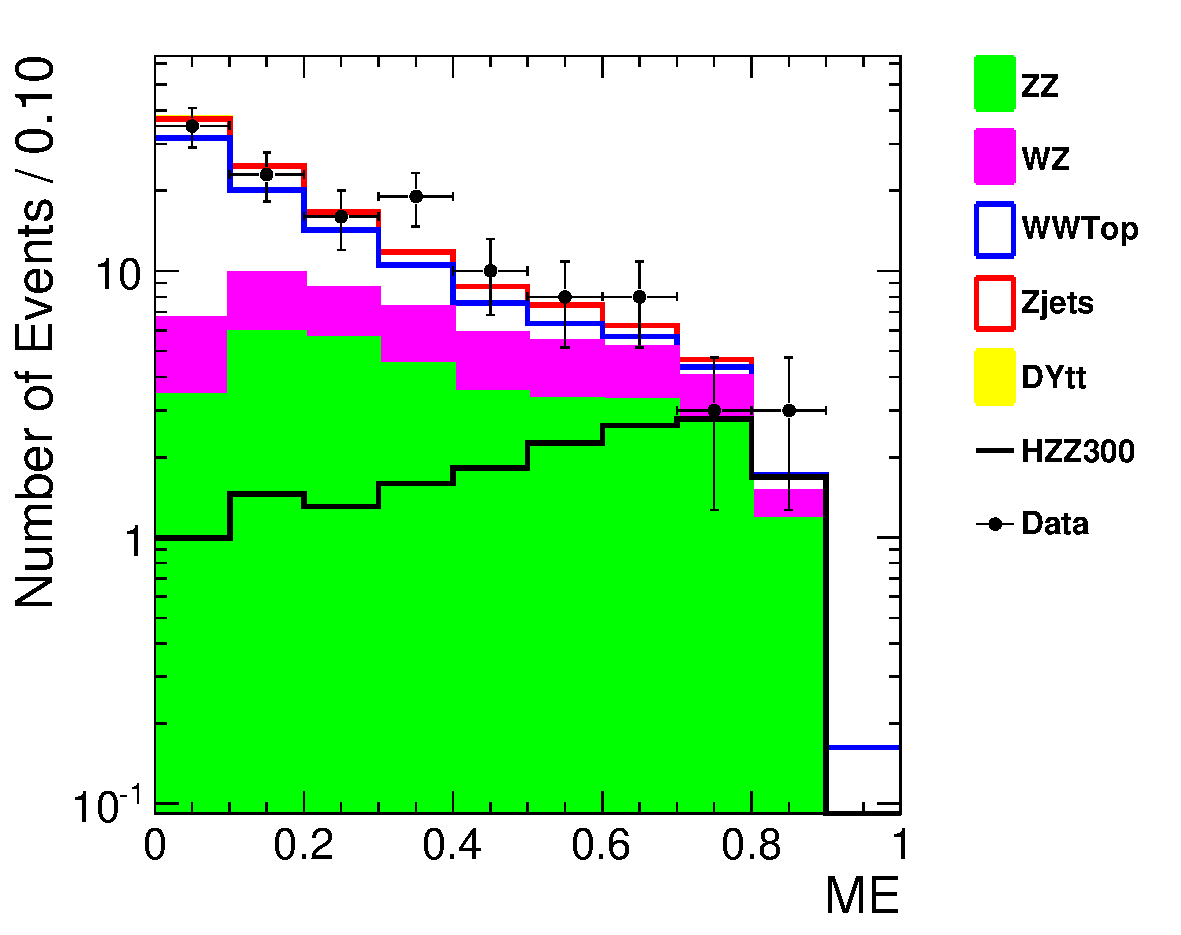
\includegraphics[width=0.4\textwidth,angle=0]{figures/ME_mH300_mm_stack_log.pdf}} \\ 
   \caption{The matrix element output distribution for Higgs signal and background events 
for \mHi=300 $\GeVcc$ in ee (a) and $\mu\mu$ final state (b) after the higgs dependent selections. 
The distributions are normalized to \intlumi with the background scaled by the data-to-mc ratios derived from data.}
   \label{fig:histo_me_300_5fb}
\end{center}
\end{figure}

\begin{figure}[!ht]
\begin{center}
   \subfigure[]{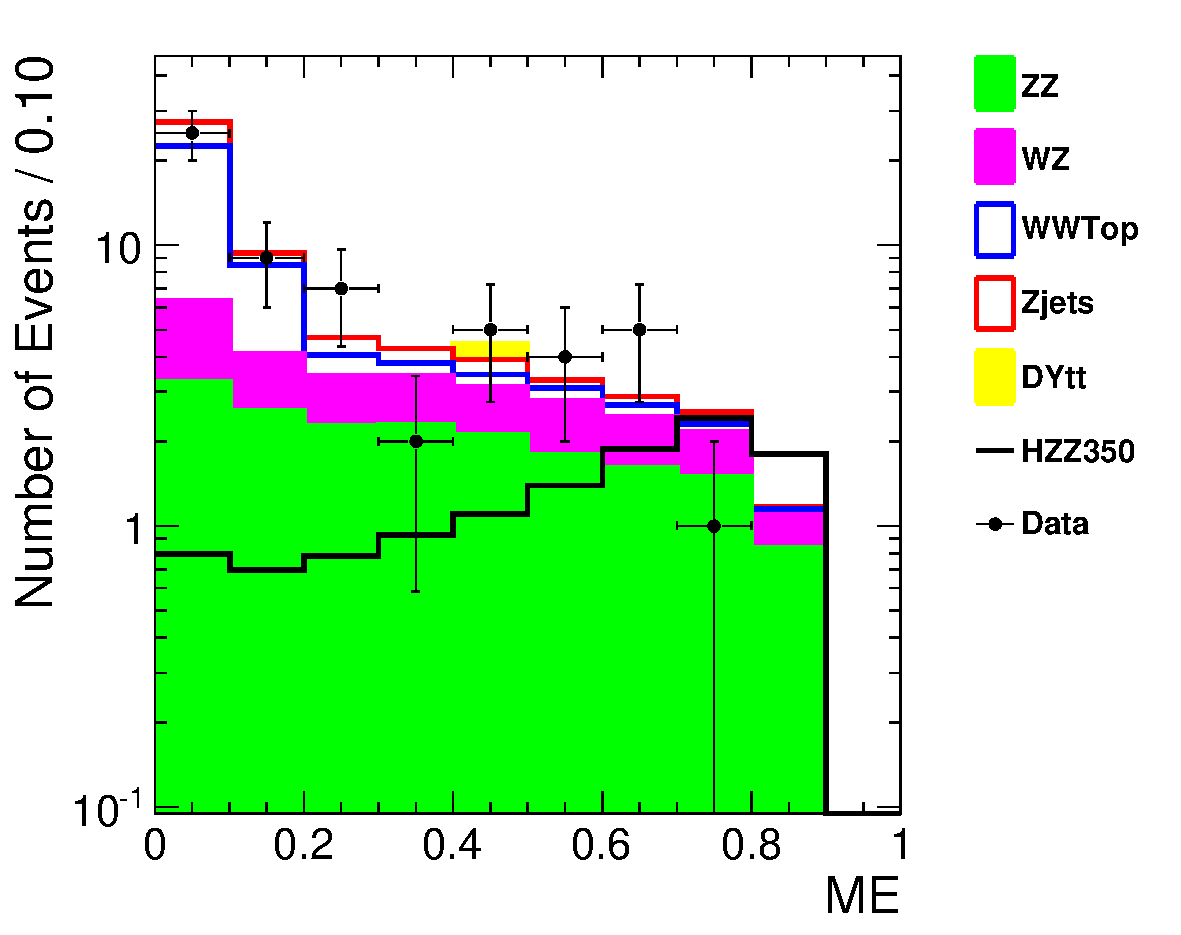
\includegraphics[width=0.4\textwidth,angle=0]{figures/ME_mH350_ee_stack_log.pdf}} 
   \subfigure[]{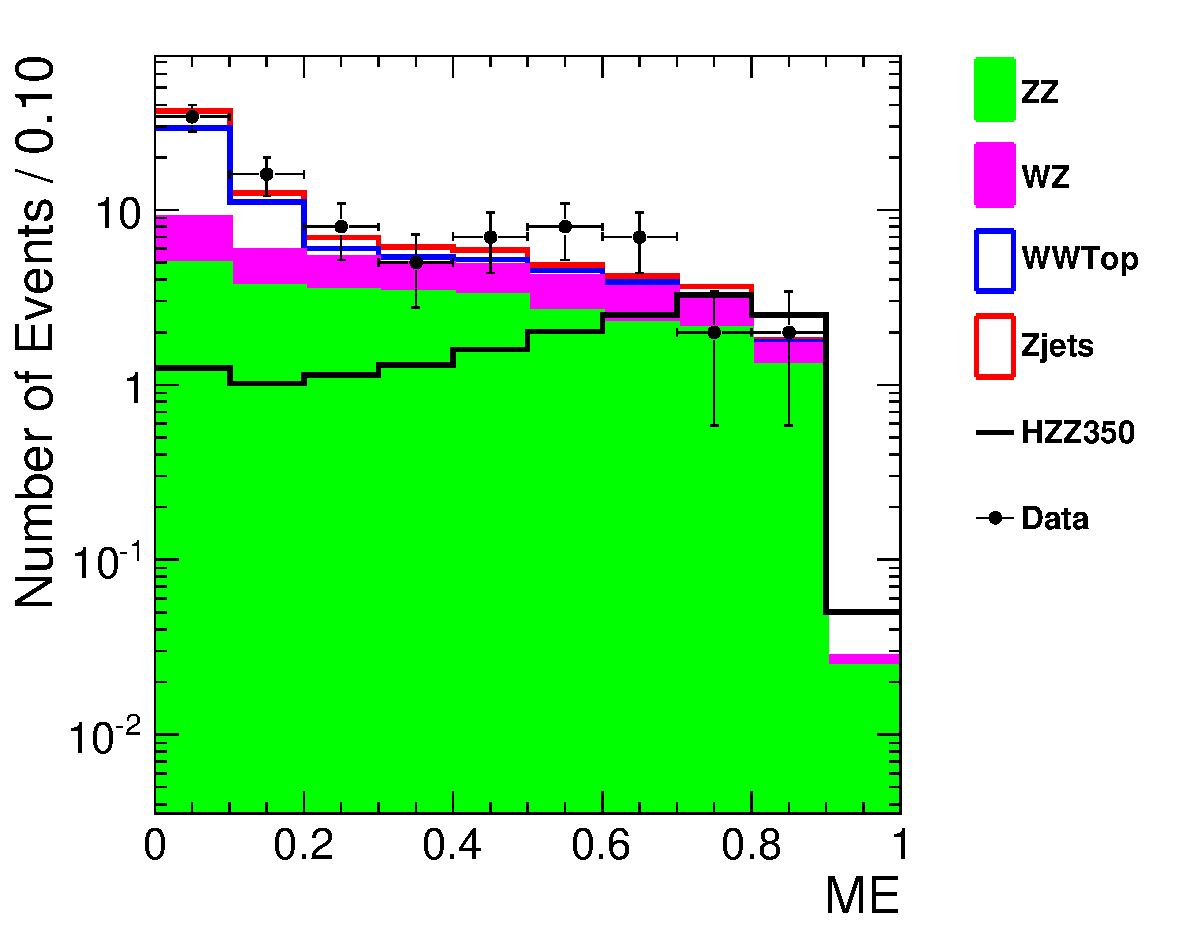
\includegraphics[width=0.4\textwidth,angle=0]{figures/ME_mH350_mm_stack_log.pdf}} \\ 
   \caption{The matrix element output distribution for Higgs signal and background events 
for \mHi=350 $\GeVcc$ in ee (a) and $\mu\mu$ final state (b) after the higgs dependent selections. 
The distributions are normalized to \intlumi with the background scaled by the data-to-mc ratios derived from data.}
   \label{fig:histo_me_350_5fb}
\end{center}
\end{figure}

\begin{figure}[!ht]
\begin{center}
   \subfigure[]{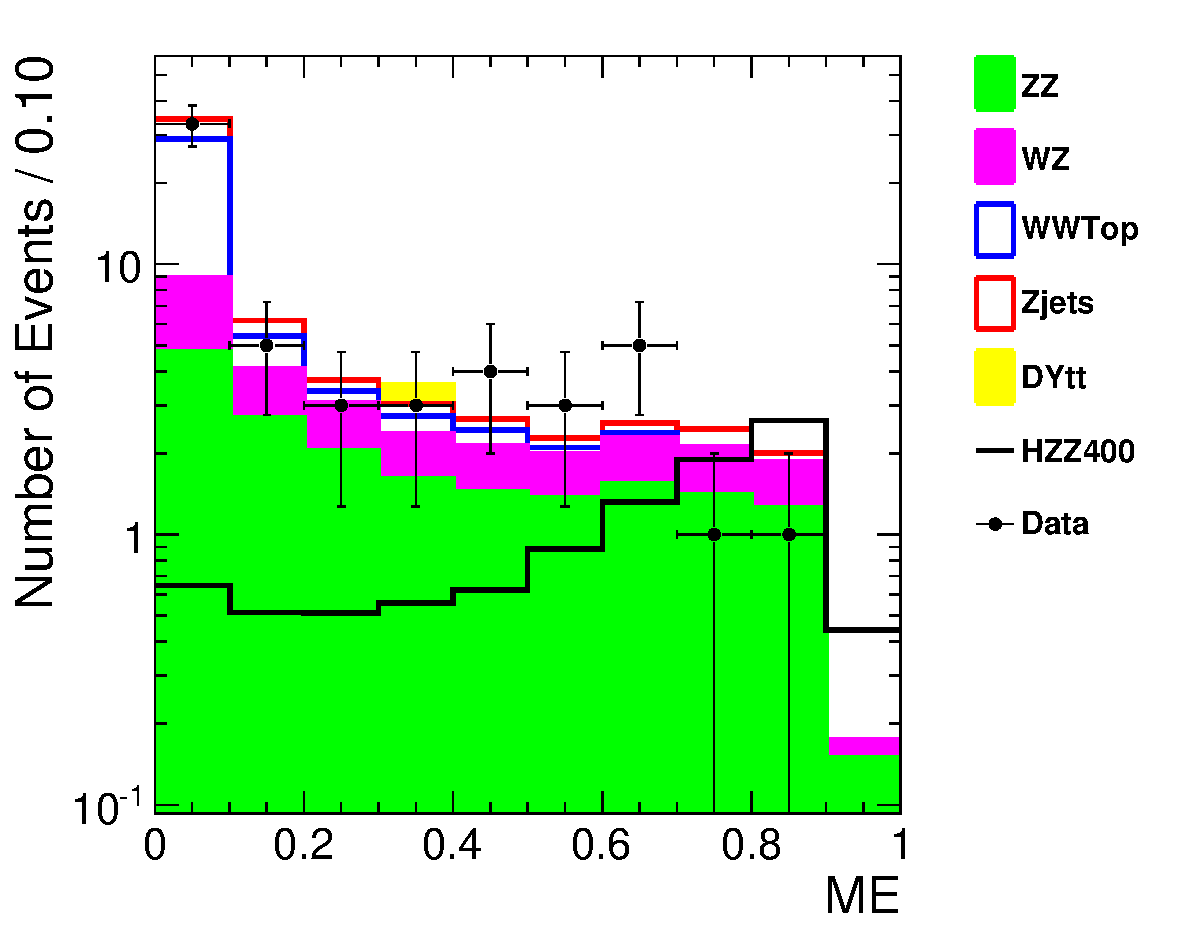
\includegraphics[width=0.4\textwidth,angle=0]{figures/ME_mH400_ee_stack_log.pdf}} 
   \subfigure[]{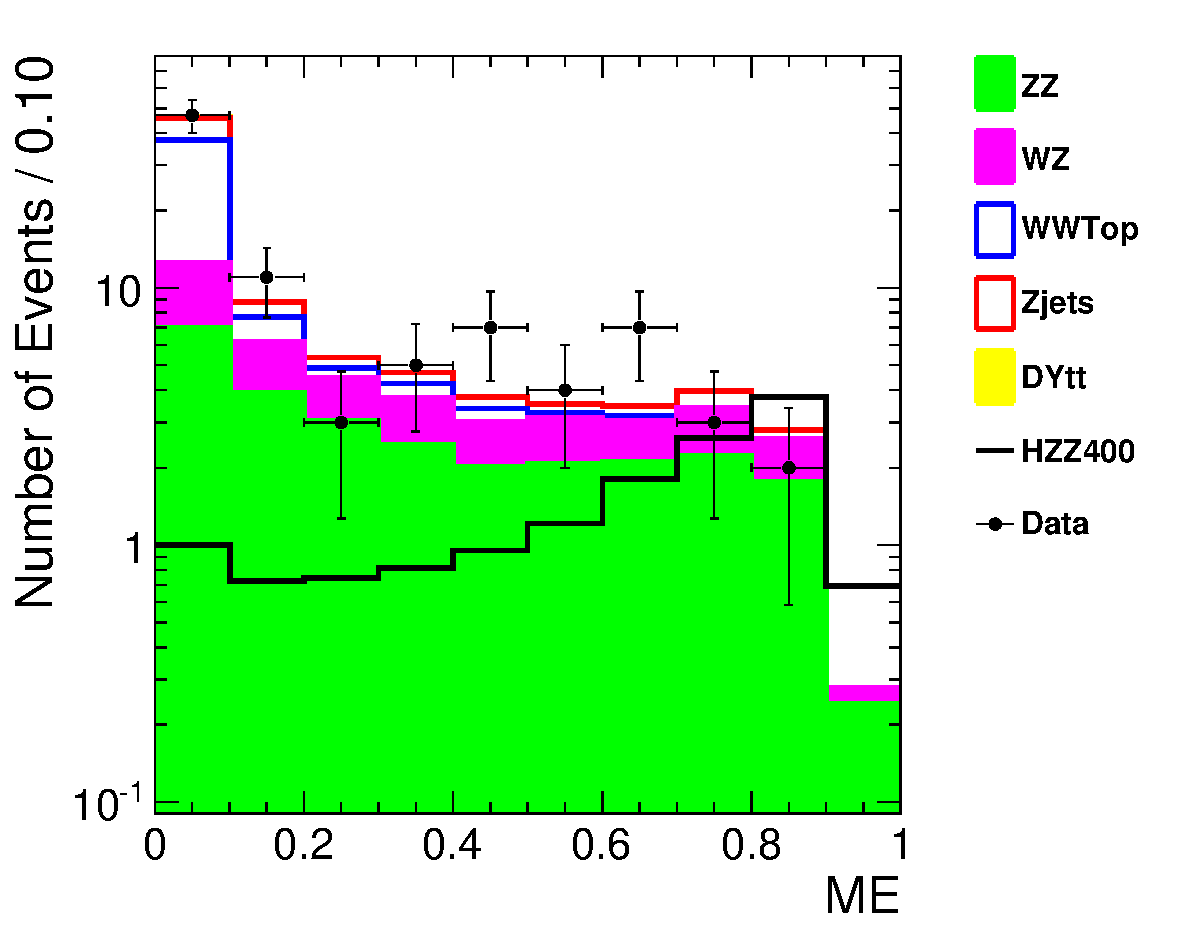
\includegraphics[width=0.4\textwidth,angle=0]{figures/ME_mH400_mm_stack_log.pdf}} \\ 
   \caption{The matrix element output distribution for Higgs signal and background events 
for \mHi=400 $\GeVcc$ in ee (a) and $\mu\mu$ final state (b) after the higgs dependent selections. 
The distributions are normalized to \intlumi with the background scaled by the data-to-mc ratios derived from data.}
   \label{fig:histo_me_400_5fb}
\end{center}
\end{figure}


\begin{figure}[!ht]
\begin{center}
   \subfigure[]{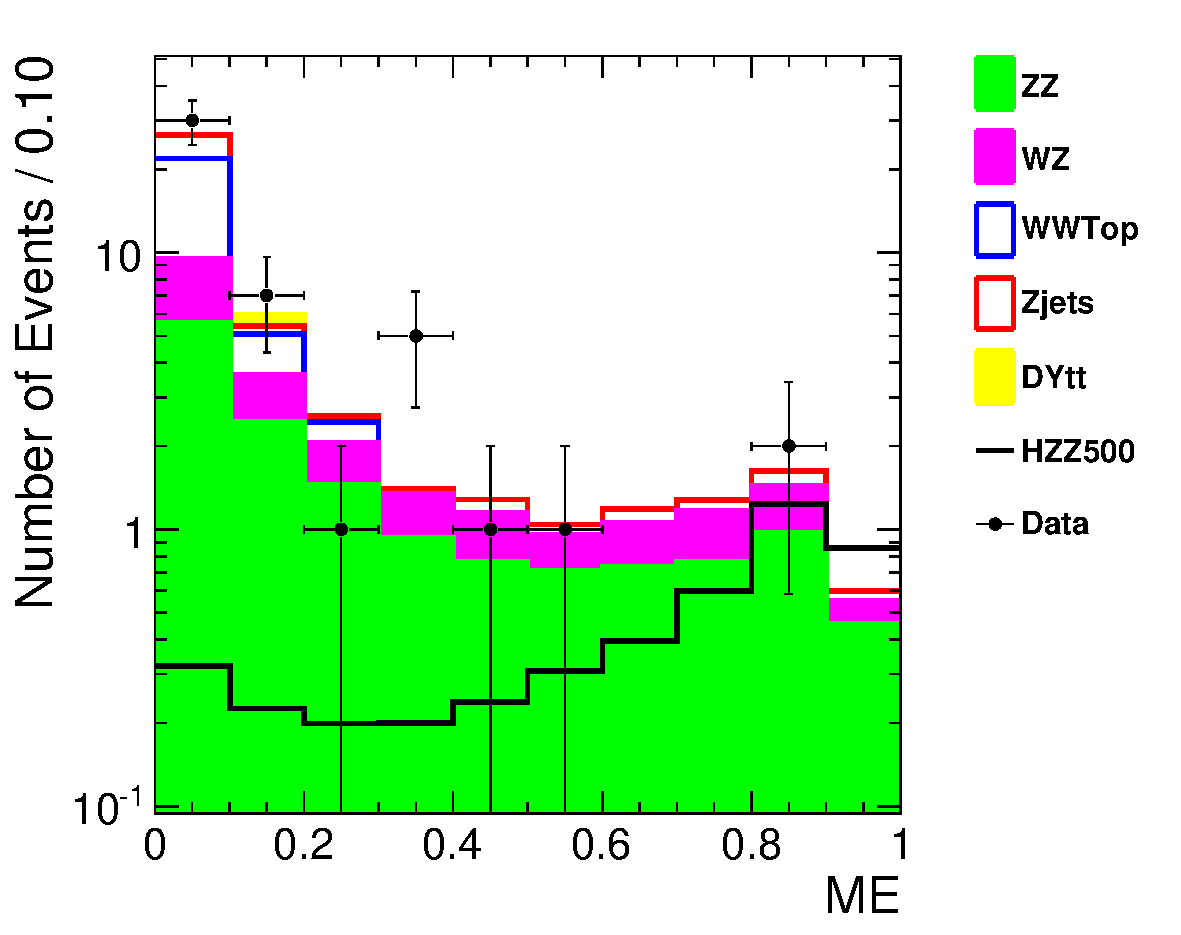
\includegraphics[width=0.4\textwidth,angle=0]{figures/ME_mH500_ee_stack_log.pdf}} 
   \subfigure[]{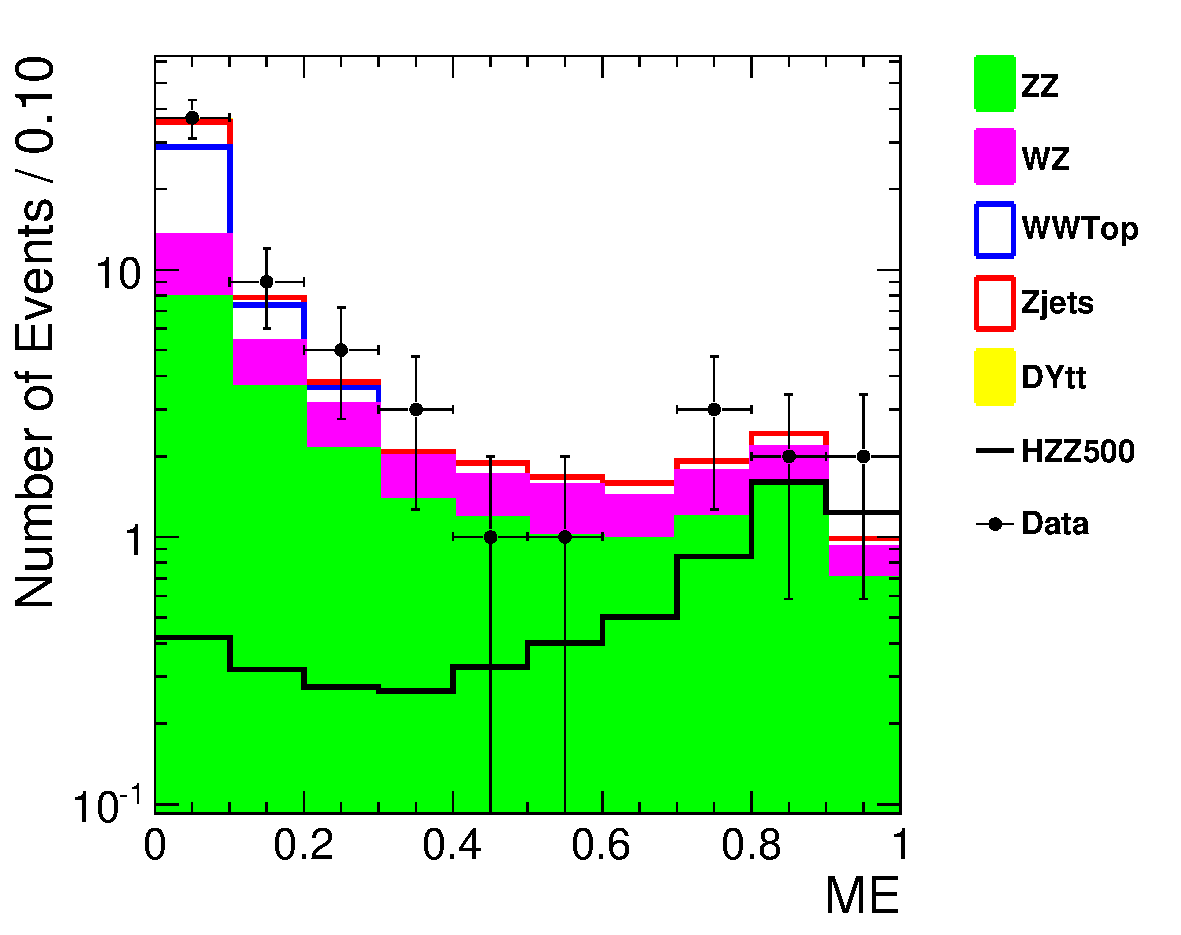
\includegraphics[width=0.4\textwidth,angle=0]{figures/ME_mH500_mm_stack_log.pdf}} \\ 
   \caption{The matrix element output distribution for Higgs signal and background events 
for \mHi=500 $\GeVcc$ in ee (a) and $\mu\mu$ final state (b) after the higgs dependent selections. 
The distributions are normalized to \intlumi with the background scaled by the data-to-mc ratios derived from data.}
   \label{fig:histo_me_500_5fb}
\end{center}
\end{figure}

\begin{figure}[!ht]
\begin{center}
   \subfigure[]{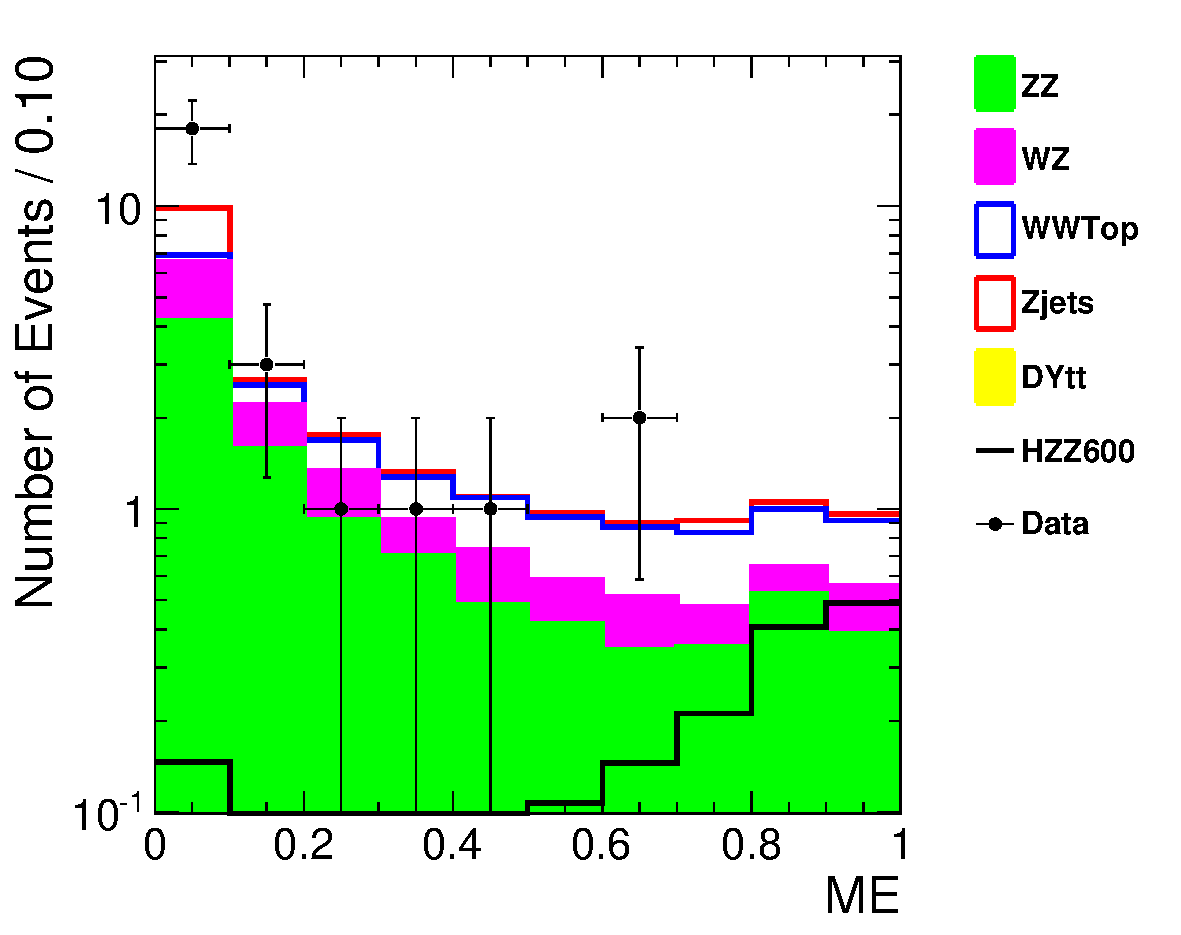
\includegraphics[width=0.4\textwidth,angle=0]{figures/ME_mH600_ee_stack_log.pdf}} 
   \subfigure[]{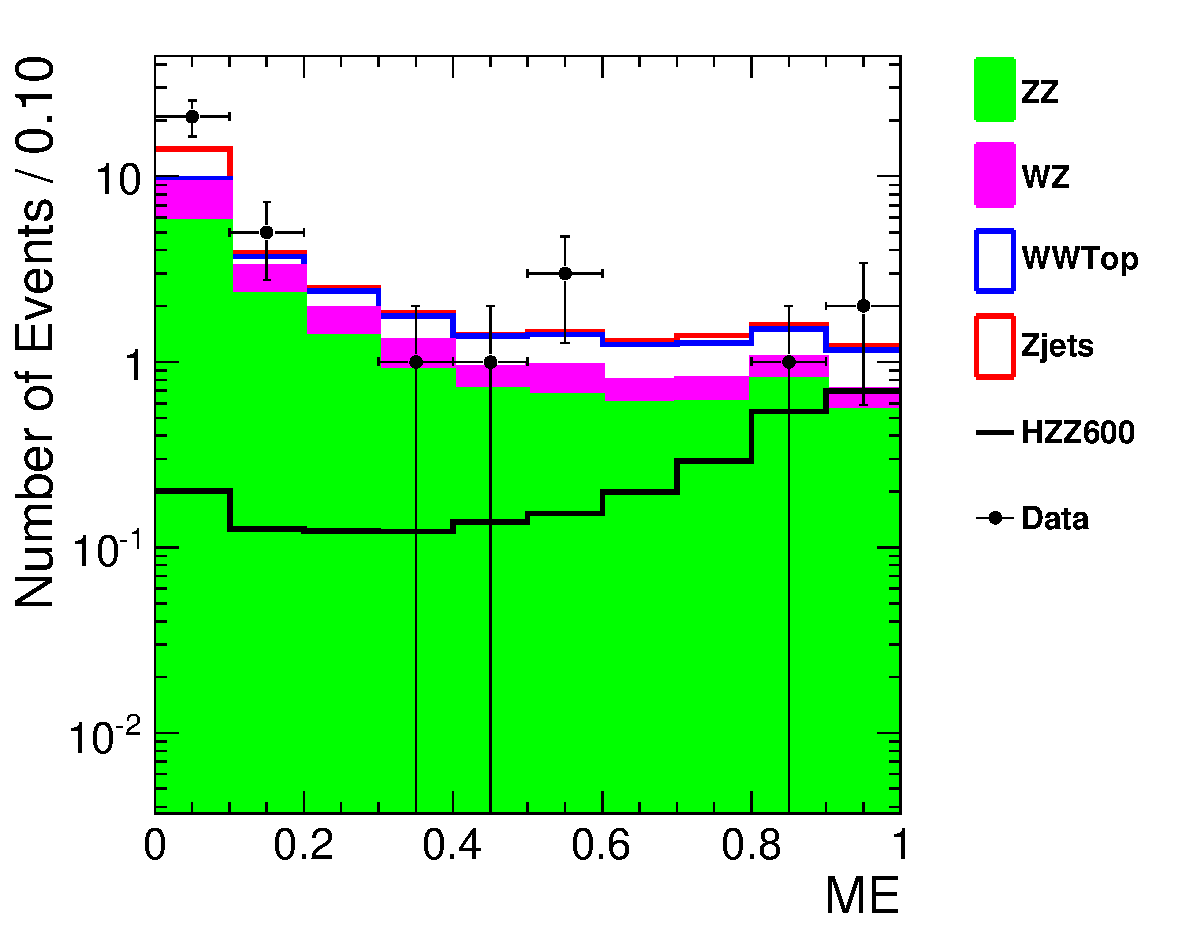
\includegraphics[width=0.4\textwidth,angle=0]{figures/ME_mH600_mm_stack_log.pdf}} \\ 
   \caption{The matrix element output distribution for Higgs signal and background events 
for \mHi=600 $\GeVcc$ in ee (a) and $\mu\mu$ final state (b) after the higgs dependent selections. 
The distributions are normalized to \intlumi with the background scaled by the data-to-mc ratios derived from data.}
   \label{fig:histo_me_600_5fb}
\end{center}
\end{figure}
%%%%%%%%%%%%%%%%%%%%%%


